\chapter{Distributed Messaging}
Messaging systems enable loose coupling and asynchronous communication between distributed components, they act as the glue binding components together.

When applied to distributed computing, messaging systems can be used to implement a wide range of communication patterns, such as request/reply, publish/subscribe, and event sourcing.
A too simplified message passing mechanism may not be enough, since it must take into account delays, message ordering, lost packets, scalability, and fault tolerance.

\section{Message Passing mechanisms}

\begin{itemize}
   \item Request-response - a client sends a request to a server, and the server sends a response back.
   \item One-way messaging - a client sends a message to a server, and the server does not send a response.
   \item Publish-subscribe - a client subscribes to a topic, and the server sends messages to all clients subscribed to that topic.
\end{itemize}


Publish-subscribe is useful because allows to receive information from multiple services, explicitly (and implicitly) categorize them, and assign them different semantics.

\subsection{Adapting Publish-subscribe to Point-to-point}
Note however that trying to create point-to-point communication with publish-subscribe may be cumbersome, and lead to un-elegant architectures, like having all clients subscribing to everyone else: a mess.

Introducing a server in the middle simplifies the topology, and allows to have a single point of contact for all clients, which forwards messages to the correct recipient.
On the other hand, it is not distributed, not scalable, and may become a bottleneck!

We could also have single queues for each client, but this is not scalable, and may lead to a single point of failure, again.

\section{Message Brokers - Kafka}
Message brokers are software systems that receive messages from producers and deliver them to consumers. They act as intermediaries between producers and consumers, and can provide additional features such as message storage, routing, and filtering.

Kafka is a distributed message broker that is designed for high-throughput, fault-tolerant, and scalable messaging. It is used in a wide range of use cases, such as log aggregation, stream processing, and event sourcing.

Messages in Kafka are similar to DB rows, and are stored in topics, which are similar to DB tables. Each message has a key, a value, and a timestamp, and is stored in a partition.

Messages are written in \textit{Batches}, which are collections of messages produced to the same topic and partition within a short time window. Batching improves throughput and reduces latency, but is a tradeoff: larger batches allows for more messages to be stored, but it might take longer for a message to be propagated.
\\


Messages are categorized into \textbf{topics}, which in turn are broken down into \textbf{partitions}, where they are written in append-only fashion and are read in order from beginning to end.
Each partition can be hosted on a different server, hence a single topic may be scaled horizontally across multiple servers to \textbf{scale-out}.


\ul{Multiple partitions imply there's not guarantee of message time-ordering across the entire topic.}

Kafka sacrifices a global order of messages for scalability, and allows to have multiple consumers reading from the same topic, and even the same partition\footnote{if they belong to different groups. This will be discussed later} at the same time.
In general it is not impossible to have a global order ---see blockchains--- but it may be very costful in a distributed environment.\\
However, \ul{if it is necessary for a topic to have a global order, it is possible to have a single partition for that topic.}

\framedt{Bypassing the Single partition limitation}{
   To avoid having a single partition but still preserve the order, we can implement some trick.

   Suppose you have a topic for ``user tracking'', with each user being identified by a key.\\
   You could create a partition for odd user IDs and one for even user IDs, and then have a single consumer for each partition.
}

\subsection{Producers and Consumers}

Producers write messages to topics, and consumers read messages from topics. Producers and consumers can be scaled horizontally to improve throughput and fault tolerance.
Scaling out consumers allows to consume message-intense topics. 

The \textbf{offset} is a unique identifier for each message within a partition, and is used by consumers to keep track of their progress. The offset is always increased, and is never reset.

Note that, in order to preserve the ordering of the message within a partition, \ul{a partition may be consumed only by one member of a consumer group at a time}.\\
In this way, the sequential semantics of a partition are preserved.\\
This implies that the maximum degree of scalability is given by the number of partitions, and not by the number of consumers.

\subsubsection{Rebalancing}
The number of partitions is set when the topic is created, and in general cannot be changed during the provisioning of the topic.\\
However, Kafka has a feature called \textit{rebalancing}, which allows to dynamically create partitions, allowing for more consumers to consume from the same topic.
However, it is a bit of a mess, and requires the provisioning to stop, compute the rebalancing plan, and then restart the provisioning.

\subsubsection{Brokers and Clusters}
A single Kafka server is called a \textit{broker}, and a group of brokers is called a \textit{cluster}. Each broker is responsible for a set of partitions, and is able to handle reads and writes for those partitions.

Brokers communicate with each other to \textbf{replicate} data and keep the cluster in sync. Each partition has a leader broker, which is responsible for handling reads and writes for that partition in the cluster. The leader broker replicates data to follower brokers, which can take over as leader if the current leader fails.

Consumers always get messages from the leader, never from the replicas, allowing to enforce asynchronous consistency.

\subsubsection{Retention}

For each topic it is possible to define a retention policy, which specifies how long messages should be retained in the topic. Messages can be retained for a fixed amount of time, or until a certain size limit is reached.

Kafka brokers are configured with a default retention
setting for topics, defining either size or time limits, which once reached, messages are deleted.


\subsubsection{Multiple Groups}

\begin{figure}[htbp]
   \centering
   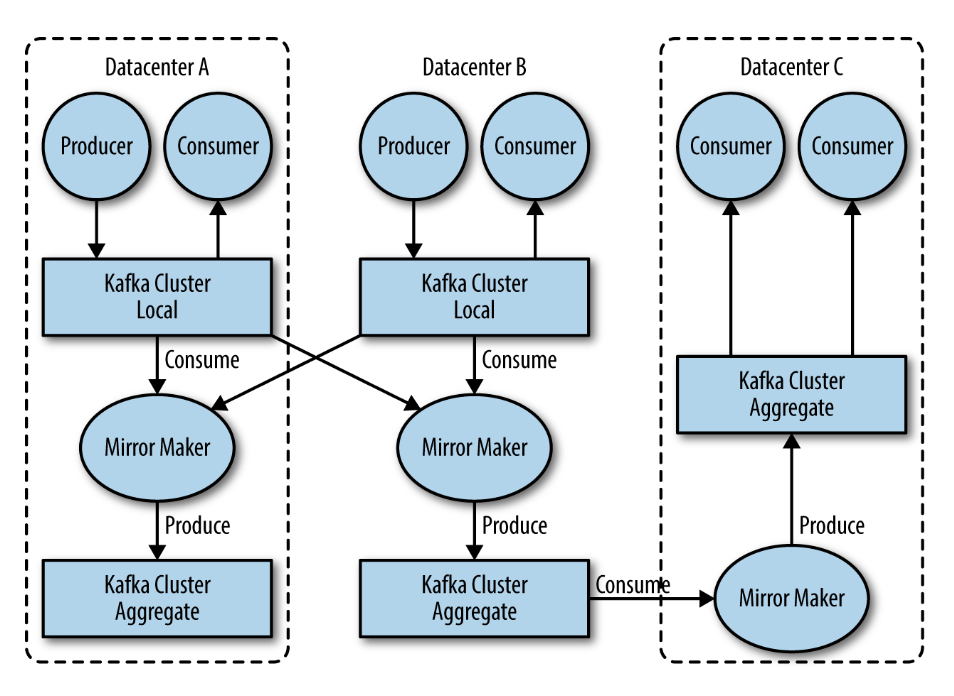
\includegraphics{images/16/clusters.png}
   \caption{Clusters and \texttt{MirrorMaker}s schema}
   \label{fig:16/clusters}
\end{figure}

As kafka deployments grow, it is often advantageous to have multiple clusters, in order to have \textbf{segregation}, \textbf{isolation}, and \textbf{fault tolerance}.

When working with multiple datacenters
it could be required that messages be
copied between them.
Kafka includes a tool called \texttt{MirrorMaker},
used for this purpose, which simply is a Kafka consumer and producer, linked together with a queue:
messages are consumed from one Kafka cluster and produced for another

\section{Using Kafka}


\subsection{Producers}
First addressing the producer point of view, it is important to consider the requirements on this side:
\begin{itemize}
   \item Is every message critical?
   \item Are accidental duplicates acceptable?
   \item Are there latency or throughput requirements?
\end{itemize}
These questions are important to correctly use the API for the producer, which can be either \texttt{fire-and-forget}, \texttt{synchronous}, or \texttt{asynchronous}.

\begin{itemize}
   \item \texttt{fire-and-forget} - the producer sends the message and does not wait for a response. Kafka automatically retries to send messages if they fail to be delivered, so most of them will be actually delivered, but some may be lost.
   \item \texttt{synchronous} - the producer sends the message and waits for a response. This is the safest way to send messages, but it is also the slowest.
   \lstinline|send()| returns a \lstinline|Future()| object, which we may invoke \lstinline|get()| on to wait for the response.
   \item \texttt{asynchronous} - the producer invokes \lstinline|send()| along with a \textit{callback} and continues with its execution.
   The callback is invoked when the message is successfully delivered, or when an error occurs.
\end{itemize}

\newpage
\subsubsection{Message record format}
\begin{paracol}{2}
   \begin{itemize}
      \item Topic
      \item Key  (optional)
      \item Partition  (optional)
      \item Value
   \end{itemize}
   
   Once sent the \texttt{ProducerRecord}, the
   producer will serialize the key and value
   objects so can be sent over the network.\\
   Later on, if a partition is
   specified in the \texttt{ProducerRecord}, the partitioner simply returns the partition we specified.
   
   A separate thread is responsible for sending those batches of records to the appropriate Kafka brokers,
   which yield a Metadata record upon successful delivery.


   \switchcolumn

   \begin{figure}[htbp]
      \centering
      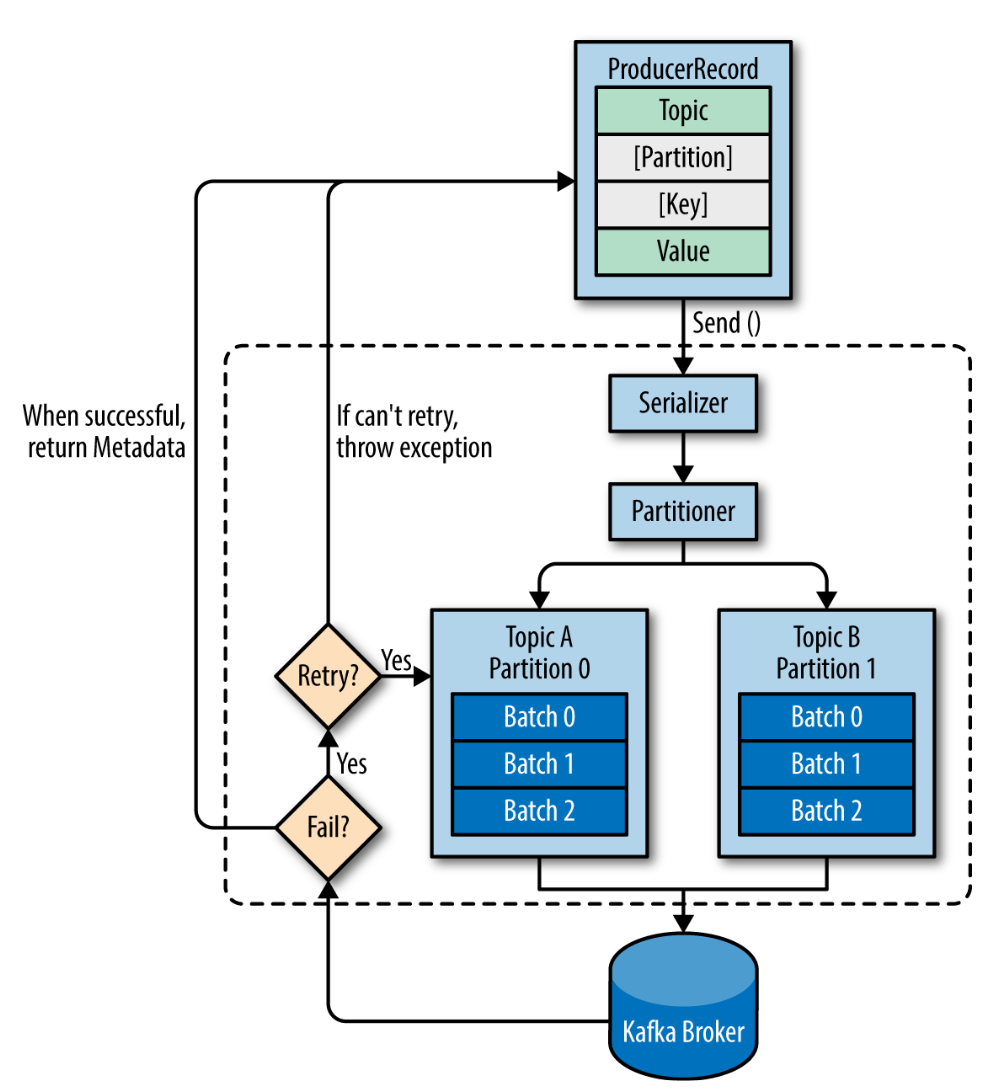
\includegraphics{images/16/producerRecord.png}
      \caption{Sending \texttt{ProducerRecord}}
      \label{fig:16/producerRecord}
   \end{figure}

\end{paracol}


\subsection{Consumers}

When dealing with Kafka messages it is important to consider that the producers may write to topics at a rate higher than the consumers can read from them.\\
This is undesirable, as it may lead to the consumers falling behind, and eventually running out of memory;
hence, we must allow to scale the consumers.

Kafka consumers are typically part of a group. When multiple consumers are subscribed to a topic and belong to the same group, each consumer in the group will receive messages from a different subset of the partitions in the topic.

\begin{figure}[htbp]
	\centering
	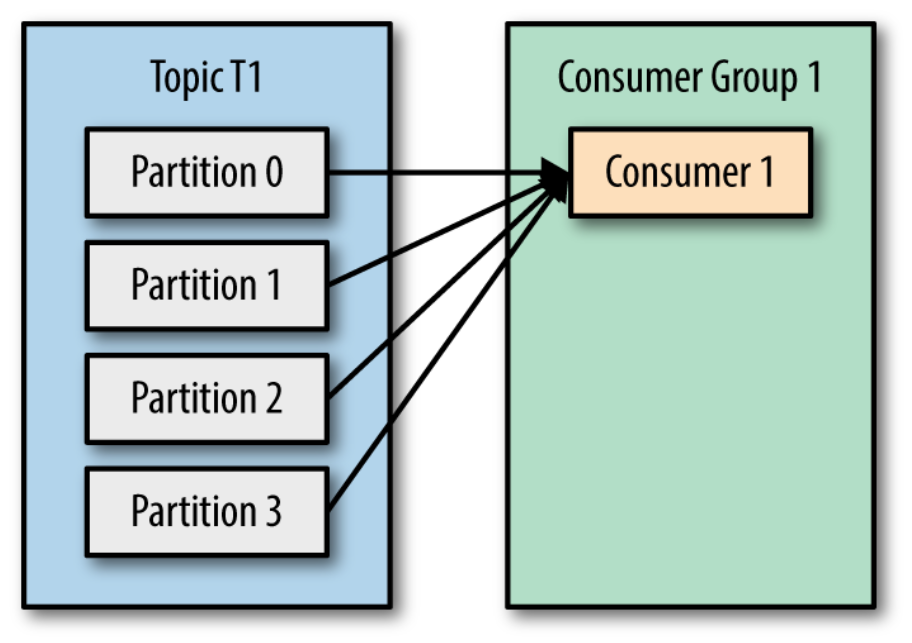
\includegraphics[width=0.3\columnwidth]{images/16/partitions_1.png}
	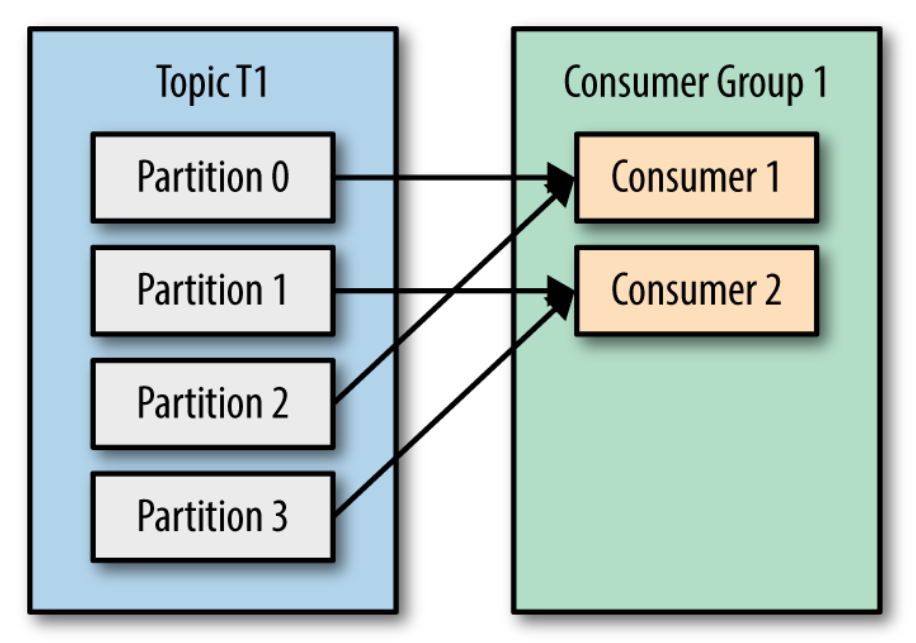
\includegraphics[width=0.3\columnwidth]{images/16/partitions_2.png}
	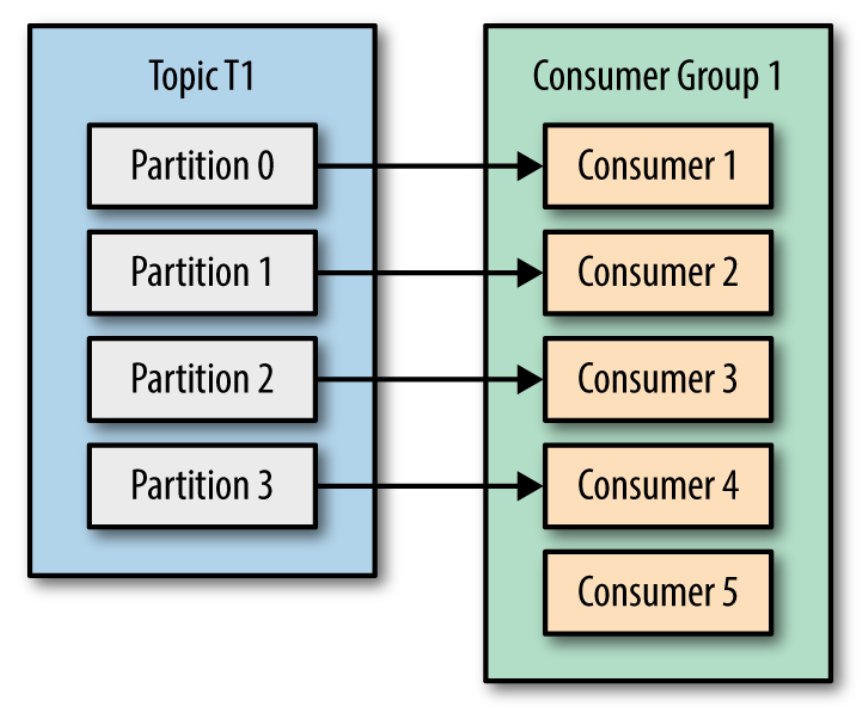
\includegraphics[width=0.3\columnwidth]{images/16/partitions_3.png}
	\caption{Partitions are assigned to Consumers to have a fair distribution.}
	\label{fig:16/partitions_1}
\end{figure}

Having more consumers than partitions is not a problem, as the consumers will simply be idle.\\
In general it is reasonable to have many partitions, allowing to scale when needed.

\begin{paracol}{2}
   It is not uncommon to have multiple applications that need to receive the same data.
   Simply assigning different consumers groups to different applications ensures that messages are delivered to all of them.
   \note{The separation among consumers remains.}
   \switchcolumn
   \begin{figure}[htbp]
      \centering
      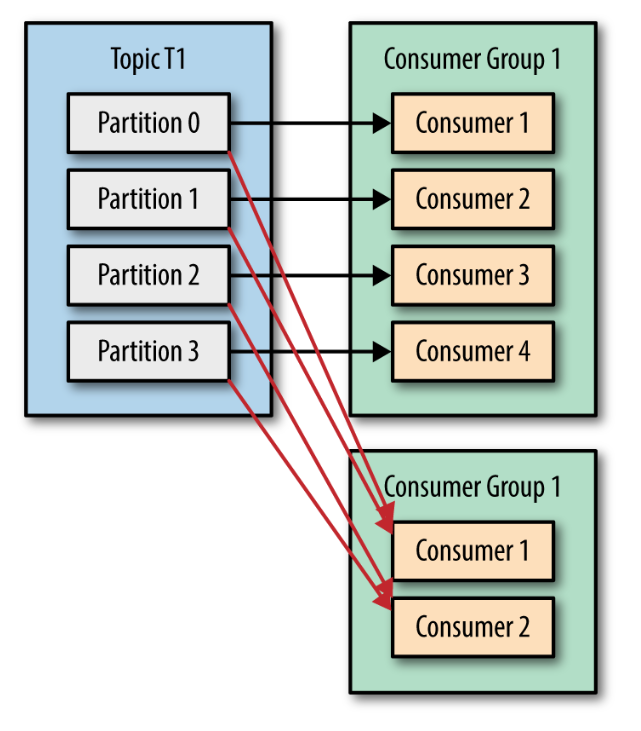
\includegraphics[width=0.5\columnwidth]{images/16/groups.png}
      \caption{Multiple Consumer Groups}
      \label{fig:16/groups}
   \end{figure}
\end{paracol}


\subsection{Rebalancing}

Moving partition ownership from one consumer to another is called a \textbf{rebalance}. Rebalances are important because they provide the consumer group with high availability and scalability,
but \ul{in the normal course of events they are \textit{fairly undesirable}}, because during a rebalance, \ul{consumers can’t consume messages}, so a rebalance is basically a short \textbf{window of unavailability} of the entire consumer group.

When partitions are moved from one consumer to another, the consumer loses its current state; if it was caching any data, it will need to refresh its caches—slowing down the application until the consumer sets up its state again.

\subsubsection{When is it needed?}
\begin{itemize}
   \item A new consumer joins the group
   \item A consumer leaves the group
   \item A consumer is considered dead
   \item The set of partitions for a topic changes
\end{itemize}

The most interesting case is when a consumer ``dies''.
If the consumer stops sending heartbeats for long enough, its session will time
out and, after a few seconds, the group coordinator will consider it ``dead'' and \ul{trigger a rebalance}.
During those seconds, no messages will be processed from the partitions owned by the dead consumer \frownie.

Instead, when closing a consumer cleanly, the consumer will notify the group coordinator that it is leaving, and the group coordinator will trigger a rebalance immediately.

\section{Kafka Strengths}
Kafka is able to seamlessly handle multiple producers, whether those clients
are using many topics or the same topic, and multiple consumers, whether they are in the same group or different groups, and also allow to seamlessly read from the same stream without interfering with each other, opposed to many queuing systems where once a message is consumed by one client, it is not available to any other.

Disk-based retention allows consumers to avoid working necessarily in real-time, and to catch up with the stream at their own pace.